\documentclass{article}

\usepackage{polski}
\usepackage{amsmath, array}
\usepackage{graphicx}
\usepackage{float}
\usepackage{subfig}
\usepackage{multirow}
\usepackage{enumitem}

\title{Laboratorium 8}
\author{\textbf{Łukasz Wala}\\
    \textit{AGH, Wydział Informatyki, Elektroniki i Telekomunikacji} \\
    \textit{Teoria Współbieżności 2022/23}}
\date{Kraków, \today}

\begin{document}
\maketitle

\section{Treść zadania}
\begin{enumerate}
    \item 
    Proszę zaimplementować przy użyciu Executor i Future program wykonujący obliczanie zbioru Mandelbrota w puli wątków.
    \item
    Proszę przetestować szybkość działania programu w zależności od implementacji Executora i jego parametrów.
\end{enumerate}

\section{Implementacja}

Poniżej znajduje się implementacja problemu dla implementacji \textit{newSingleThreadExecutor},
czyli executora z tylko jednym dostępnym wątkiem. Zadanie zostało podzielone tak, że każdy z wątków
ma do wykonania działania dla jednego wiersza pixeli w obrazie.

\begin{verbatim}
class MandelbrotCallable implements Callable<Integer> {
    private BufferedImage image;
    private int maxIter;
    private double zoom;
    private int y;
    private int maxWidth;

    private double zx, zy, cX, cY, tmp;

    public MandelbrotCallable(BufferedImage image, int maxIter, double zoom, int maxWidth, int y) {
        this.image = image;
        this.maxIter = maxIter;
        this.zoom = zoom;
        this.maxWidth = maxWidth;
        this.y = y;
    }

    public Integer call() {
            for (int x = 0; x < maxWidth; x++) {
                zx = zy = 0;
                cX = (x - 400) / zoom;
                cY = (y - 300) / zoom;
                int iter = maxIter;
                while (zx * zx + zy * zy < 4 && iter > 0) {
                    tmp = zx * zx - zy * zy + cX;
                    zy = 2.0 * zx * zy + cY;
                    zx = tmp;
                    iter--;
                }
                image.setRGB(x, y, iter | (iter << 8));
            }

        return 0;
    }
} 

class MainExecutor extends JFrame {
    private BufferedImage image;
    
    private final int MAX_ITER = 570;
    private final double ZOOM = 150;

    public MainExecutor() {
        super("Mandelbrot Set with Executor");
        setBounds(100, 100, 800, 600);
        setResizable(false);
        setDefaultCloseOperation(EXIT_ON_CLOSE);
        image = new BufferedImage(getWidth(), getHeight(), BufferedImage.TYPE_INT_RGB);

        ExecutorService executor = Executors.newSingleThreadExecutor();
        List<Future<Integer>> futures = new ArrayList<>();

        for (int y=0; y<getHeight(); ++y) {
            MandelbrotCallable callable = new MandelbrotCallable(image, MAX_ITER, ZOOM, getWidth(), y);
            Future<Integer> future = executor.submit(callable);
            futures.add(future);
        }

        for(Future<Integer> future : futures) {
            try {
                future.get();
            } catch (ExecutionException | InterruptedException e) {
                System.exit(1);
            }
        }
    }   

    @Override
    public void paint(Graphics g) {
        g.drawImage(image, 0, 0, this);
    }

    public static void main(String[] args) {
        new MainExecutor().setVisible(true);
    }
}    
\end{verbatim}

\section{Porównanie szybkości}

W celu wydłużenia czasu działania programu dla wszystkich przypadków podniesiona zostanie wartość \textit{MAX\_ITER} do 10000.

Dla \textit{newSingleThreadExecutor}, w którym nie ma możliwości manipulacji liczbą wątków z oczywistych względów, czas działania wynosi 1497 ms.

Dla \textit{newCachedThreadPool}, który tworze więcej nowych wątków w zależności od potrzeb i używa ponownie starych wątków, czas wykonania wynosi 284 ms.
Czas działania jest zauważalnie niższy, niż dla pojedynczegi wątku, czego można było się spodziewać.

Poniżej wykres porównani czasu działania od liczby wątków dla implementacji \textit{newFixedThreadPool}, która używa puli wątków o konkretnym, ustalonym rozmiarze:
\textit{newWorkStealingPool} (użyta liczba wątków od 1 do 8, bo tylko tyle fizycznych wątków posiada maszyna używana do testowania):

\begin{figure}[H]
    \centering
    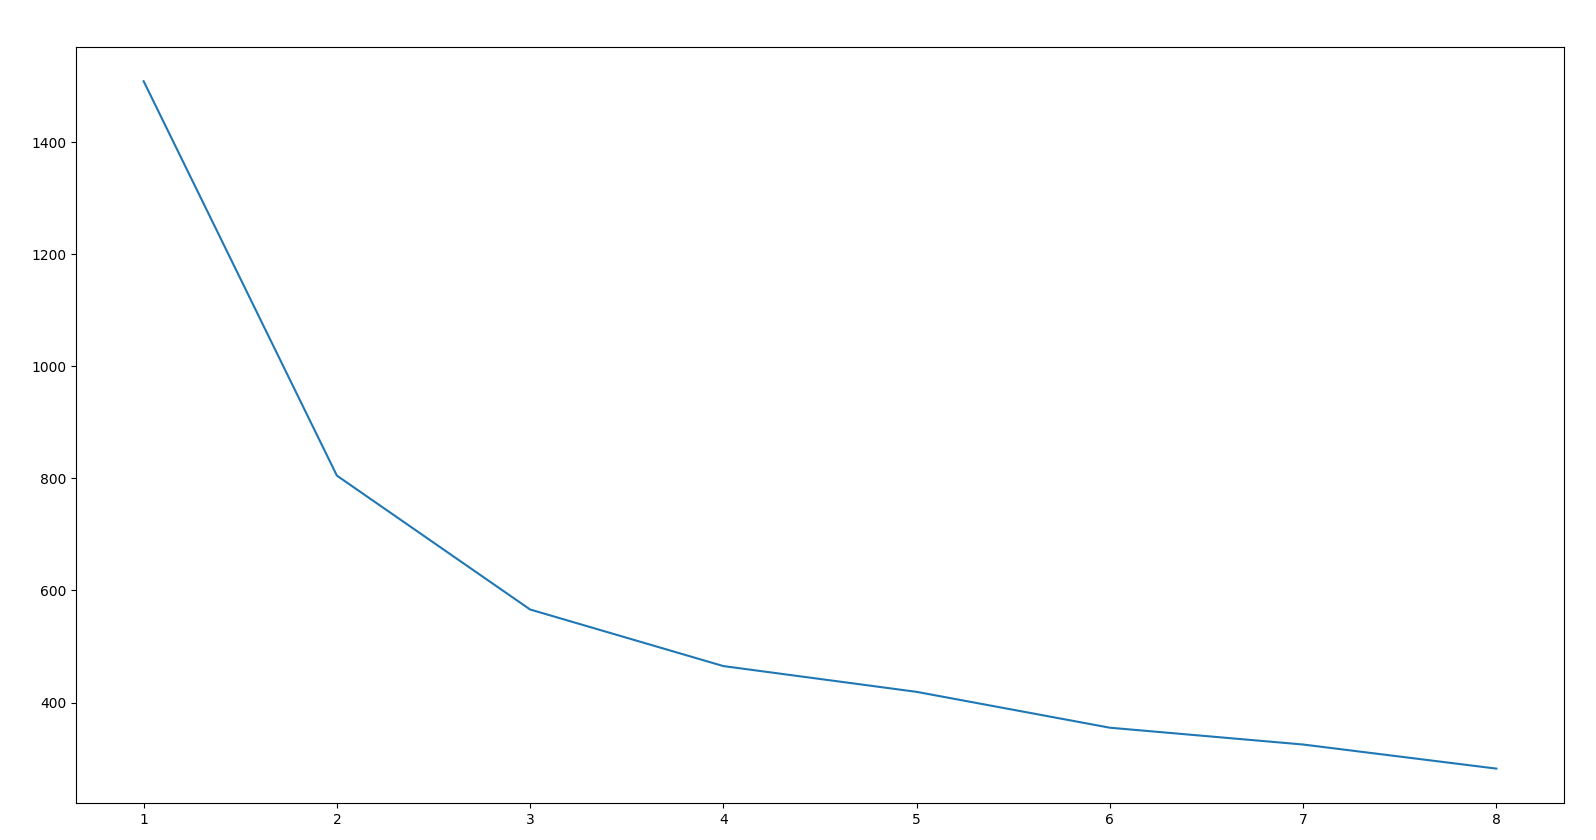
\includegraphics[width=\textwidth]{figure_1.png}
    \caption{Wykres porównania dla \textit{newFixedThreadPool}}
\end{figure}

Warto zauważyć, że dla ośmiu wątków czas działania był porównywalny do \textit{newCachedThreadPool}, co może sugerować, 
że ten drugi używał wszystkich dostępnych (czyli ośmiu) wątków.

Implementacja \textit{newWorkStealingPool} używa parametru \textit{parallelism}, czyli \textit{poziomu równoległości},
w zależności od którego zależy dynamicznie zmieniająca się liczba używanych wątków, poniżej wykres dla kilku wartości:

\begin{figure}[H]
    \centering
    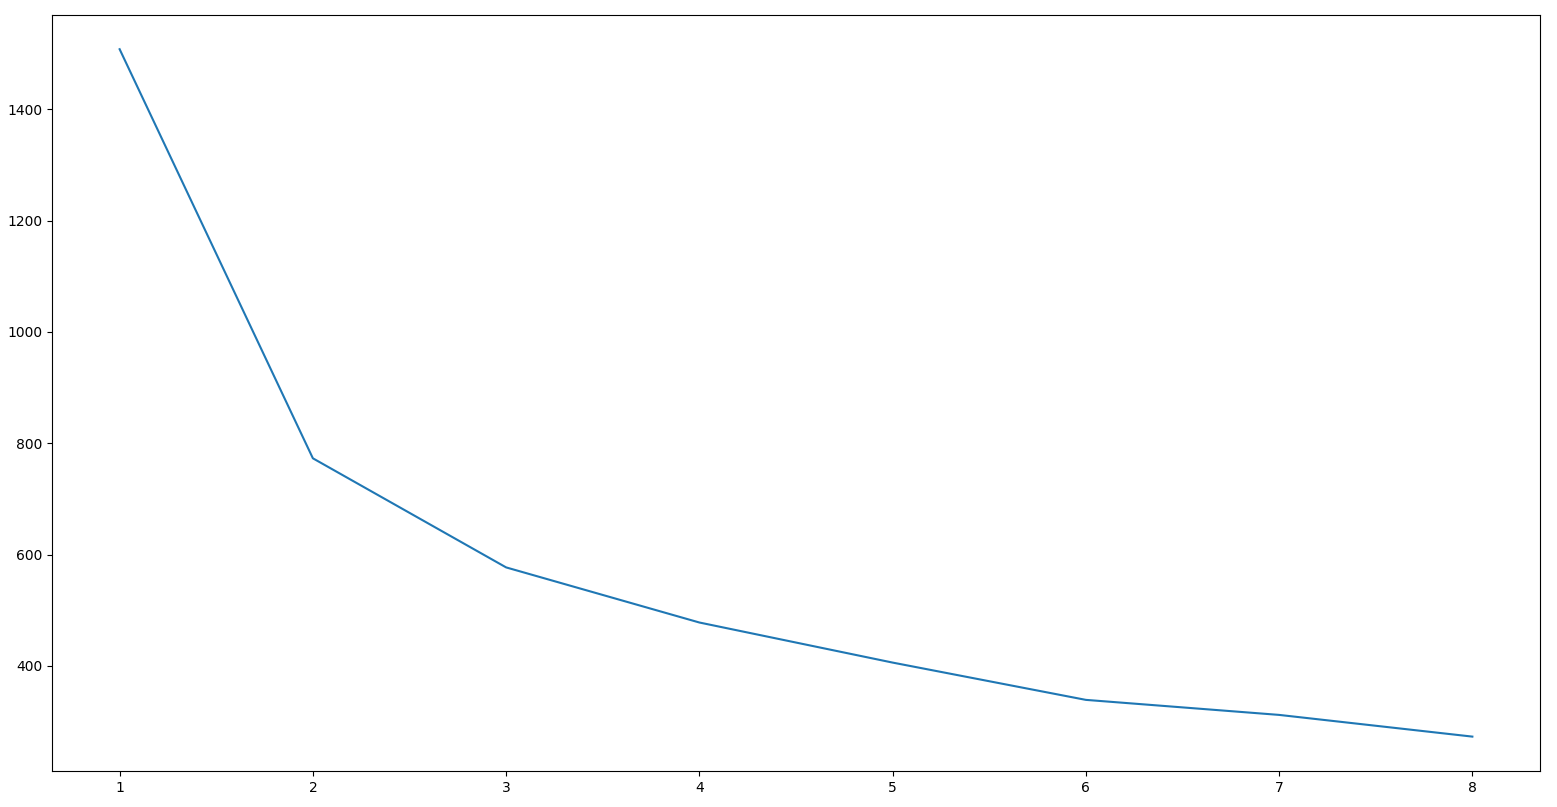
\includegraphics[width=\textwidth]{figure_2.png}
    \caption{Wykres porównania dla \textit{newWorkStealingPool}}
\end{figure}

Wyniki są bardzo podobne jak w przypadku \textit{newFixedThreadPool}, co pozwala wnioskować, że dla danych poziomów
używane są podobne liczby wątków.

\section{Wnioski}

Interfejs \textit{Callable} umożliwia wątkom zwracanie wartości, co jest przydatne, gdy wątki wykonują pewne
obliczenia, które trzeba zwrócić przy uniknięciu manipulowania dzielonym stanem.

\textit{ExecutorService} pozwala na łatwe uruchamianie pewnej liczby wątków, jego różne implementacje pozwalają
na używanie pojedynczego wątku, pewnej ustalonej liczby lub dynamicznie zmieniającej się liczby zależnej od 
potrzeb, co pozwala na efektywne wykorzystywanie zasobów.

\section{Bibliografia}

\begin{enumerate}
    \item 
    Dokumentacja języka Java - docs.oracle.com
\end{enumerate}

\end{document}